\section{Mini-projet d'e-banking}

À la suite de notre formation, nous avons mis en pratique nos connaissances dans un mini-projet de réalisation d'une application web d'e-banking.

\subsection{Cahier des charges}

L'application à réaliser est une application web de gestion des comptes. Les fonctionnalités sont les suivantes :

\begin{itemize}
	\item S'identifier,
	\item Consulter la liste de ses comptes,
	\item Consulter le détail des opérations pour un compte et un mois donné,
	\item Consulter le détail des opérations cartes pour un compte et un mois donné,
	\item Effectuer un virement entre ses comptes,
	\item Consulter l'historique de ses virements,
	\item Exposer ces fonctionnalités sous la forme de web services.
\end{itemize}

\subsection{Gestion du projet}

Étant 9 stagiaires à être arrivé le même jour et un autre la semaine suivante, nous nous sommes tout d'abord divisé en deux groupes de 5 stagiaires, chaque groupe réalisant sa propre version de l'application. La séparation en groupe s'est faite de façon complètement aléatoire.\\

La méthode que nous avons utilisé pour gérer ce projet est un mélange entre la méthode Scrum et XP, soit deux méthodes Agiles. L’utilisation des méthodes Agiles repose en grande partie sur le constat qu’un produit logiciel voit la plupart du temps ses demandes en fonctionnalités évoluer au fur et à mesure, et que cela est très difficile à prendre en compte avec un simple système en une itération, c'est à dire, en utilisant pas exemple le cycle en V. Ici, le but est d’effectuer de courtes itérations d’une à deux semaines au bout desquelles un produit utilisable est livré. Dans notre cas nous avons fait des itérations (ou sprints) d'une semaine.\\

La première itération, appelé Sprint 0 a consisté en la mise en place de l'environnement de développement, de l'environnement d'intégration ainsi que des conventions à utiliser. C'est au cours de cette semaine que nous avons aussi choisi les technologies à utiliser. Nous avons aussi réfléchi à l'architecture générale de l'application. Tous ces choix sont expliqué un peu plus loin dans le rapport. À la fin de ce premier Sprint, nous avons fait une réunion avec Stéphane LANDELLE, le directeur technique d'\ebi{}, pour avoir un avis sur nos choix.\\

Les autres itérations ce sont toutes déroulées de la même façon :
\begin{enumerate}
	\item Réunion avec le \flqq{}product owner\frqq{} (client dans le vocabulaire Scrum), c'est à dire Stéphane, pour sélectionner les fonctionnalités à développer dans cette itération,
	
	\item Développement des fonctionnalités en pair programming pour mutualiser les connaissances,
	
	\item Réunion avec Stéphane pour auditer notre code et pour présenter le résultat de l'itération,
	
	\item Remaniement (refactoring) du code suite aux remarques de Stéphane.\\
\end{enumerate}

De plus, chaque jour nous faisions un \flqq{}daily Scrum\frqq{} entre nous : c'est une courte réunion dans laquelle tout les intervenants sont debout (pour se forcer à faire court) et résument ce qu'ils ont fait la veille en mentionnant les problèmes rencontrés.\\

Cette méthode permet d'avoir un résultat chaque semaine à montrer au client. Le client peut donc voir l'évolution du projet en temps réel, tester les parties déjà développées ce qui permet d'avoir un retour. De plus, le client est beaucoup plus intégré au projet et peut facilement ajuster ou modifier le cahier des charges.\\

Pour le développeur, les itérations permettent de ne pas avoir un travail trop répétitif puisque dans chaque itération, on retrouve toutes les phases du cycle en V classique. Il n'y a donc plus de grandes phases de développement, de tests, de recette, \dots{}

\subsection{Choix techniques}

Le choix des technologies à utiliser était libre, même s'il était soumis à l'approbation de Stéphane. Voici les technologies que nous avons choisi :

\subsubsection{Gestionnaire de version}

Il permet de travailler sur un projet de manière collaborative en versionnant le code pour pouvoir facilement revenir à une version antérieure. Il existe principalement deux gestionnaires de version : Git et Subversion.\\

Subversion est le plus répandu actuellement car plus vieux. Il est robuste et à fait ses preuves depuis longtemps. Le développement est linéaire. Git, lui, est assez récent (2005). Il tire profit au maximum des branches pour avoir des fonctionnalités se développant en parallèle sans rentrer en conflit. Une fois une fonctionnalité développée sa branche est fusionnée à la branche principale (master).\\

Nous avons choisi d'utiliser Subversion, car c'est celui qui est le plus utilisé. Ça nous a permis de nous faire la main dessus pour être prêt à l'utiliser en clientèle. Pour que notre projet soit accessible de n'importe où, nous avons choisi d'utiliser Google Code \cite{capicsou-bank-svn} pour héberger notre dépôt Subversion.

\subsubsection{Construction du projet}

Plusieurs systèmes permettent de construire des projets Ant, Maven, Gradle, \dots{} Ant est le plus ancien. C'est globalement un outil qui permet d'écrire des scripts pour construire des applications. Il est très apprécié car il est très flexible.\\

Maven est plus récent et se base sur le principe de \flqq{}convention over configuration\frqq{}, c'est à dire qu'il encourage le développeur à respecter certaines conventions pour faciliter la construction du projet comme par exemple l'emplacement des sources et celui des sources des tests. Il inclut aussi un système de gestion de dépendance qui va directement chercher les librairies externes dans des dépôts Maven accessibles à tout le monde.\\

Gradle quant à lui est le plus récent. Il reprend beaucoup des principes de Maven, notamment la gestion des dépendances. Mais il se comporte plus comme Ant dans la mesure où il reste très flexible.\\

Nous avons choisi Maven car il est celui qui nous semble le plus abouti.

\subsubsection{Système de Gestion de Base de Données (SGBD)}

Afin de persister nos données nous avons besoin d'un SGBD. Il existe de nombreuses possibilités et l'application à réaliser n'a pas besoin de fonctionnalités avancées hormis une gestion des transactions pour garantir la cohérence de nos tables.\\

Les deux principaux SGBD open source sont MySQL et PostgreSQL. Ces deux solutions sont assez proches. Nous avons choisi MySQL puisque c'est celui le plus utilisé entre ces deux SGBD.

\subsubsection{ORM}

Hibernate s'est imposé de lui-même pour gérer la persistance de nos objets dans notre SGBD car il est le plus utilisé. De plus, c'est celui sur lequel nous avons été formé.

\subsubsection{Conteneur d'application}

Les conteneurs d'applications sont des boites à outils fournissant des services pour résoudre des problématiques que toute application rencontre. Dans le monde Java, il en existe principalement deux : JEE et Spring.\\

Nous avons décidé d'utiliser Spring pour son aspect conteneur léger. En effet, notre application n'a pas besoin des fonctionnalités d'un serveur tel que Glassfish ou WebLogic reconnu pour être des conteneurs lourds. Avec Spring, l'application peut se déployer dans un serveur léger tel que Tomcat qui n'implémentent que les spécification Servlet et JSP, soit le strict minimum pour une application web.\\

De plus, Spring permet de facilement intégrer Hibernate et de simplifier la réalisation d'une application web avec son module Spring MVC.

\subsubsection{Serveur}

Puisque nous utilisons Spring, nous pouvons utiliser un serveur léger. Il en existe surtout deux Jetty et Apache Tomcat. Nous avons préféré Tomcat car encore une fois, il est le plus répandu.

\subsubsection{Frameworks de tests}

Afin de tester notre application nous avons décider d'utiliser plusieurs frameworks de tests. Tout d'abord, pour les tests unitaires, nous avons utilisé JUnit. Une autre possibilité aurait été d'utiliser TestNG mais il est beaucoup moins répandu.\\

Nous avons aussi utilisé un framework de mock pour \flqq{}mocker\frqq{} nos objets lors de nos tests. Mocker un objet consiste à remplacer un objet par un faux dont on fixe le comportement. Si par exemple une classe A utilise une autre classe B pour son fonctionnement. Lorqu'on veut tester uniquement la classe A, il faut mocker la classe B et injecter le mock dans la classe A. Ainsi les bugs dans la classe B n'interfèrent pas avec les tests de la classe A. Pour cela nous avons utilisé Mockito qui nous a été recommandé par Stéphane. Les autres possibilités sont EasyMock ou PowerMock.\\

Enfin, pour les tests d'intégration, nous avons utilisé Selenium. Les tests d'intégration sont des tests au niveau qui testent l'interface et vérifient le bon fonctionnement de l'application finale. Ces tests sont plus lourds et exécuté non pas par le développeur mais par le serveur d'intégration.

\subsubsection{Serveur d'intégration}

Un serveur d'intégration est un serveur qui périodiquement récupère le code source d'un projet depuis un gestionnaire de version, le construit, exécute les tests unitaires et les tests d'intégrations et génère un rapport avec le résultat de la construction du projet et de l'exécution des tests. Ce serveur permet d'avoir un système d'intégration continue : lorsqu'un développeur modifie le code source et envoie ses modifications au gestionnaire de version, le serveur d'intégration va permettre de vérifier qu'il n'y ait pas de régression et garantir le bon fonctionnement de l'application.\\

Nous avons choisi d'utiliser Jenkins (appelé Hudson auparavant) car c'est le seul serveur d'intégration open source que l'on connaisse. Ce serveur fonctionnait sur un des postes des stagiaires et récupérait régulièrement les sources depuis notre dépôt Subversion pour ensuite construire notre projet et exécuter les tests unitaires et les tests d'intégration.

\subsubsection{Framework de web services}

Les web services sont des services distribués utilisant HTTP comme protocole de transport. Ces web services permettent à une application tierce d’interagir avec notre application. Il existe principalement deux types de web services : SOAP (Simple Object Access Protocol) et REST (REpresentational State Transfer).\\

SOAP s'appuie principalement sur XML ce qui fait de lui un protocole très verbeux et est généralement utilisé dans un même réseau, c'est à dire entre des applications d'un même système d'information par exemple.\\

REST n'est pas à proprement parlé un protocole mais simplement un principe : puisqu'on utilise HTTP pour le transport, utilisons toutes les possibilités de ce protocole. Il est généralement utilisé en combinaison avec JSON (JavaScript Object Notation) permettant de représenter les objets sous la forme de chaîne de caractères.\\

Pour la mise en place des web services nous avons choisi Apache CXF puisqu'il permet de faire des web services SOAP et REST et s'intègre complètement avec Spring.

\subsubsection{Autres technologies}

Nous avons utilisées d'autres technologies sur lesquelles je ne m'étendrai pas sur le choix :

\begin{description}
	\item[JSTL] Fourni un ensemble de tags pour faciliter l'écriture de pages JSP avec notamment des boucles et des blocs conditionnelles tout en restant complètement du code XML,
	
	\item[Flyway] Permet de versionner la base de données en écrivant des scripts de migration s'exécutant lors du déploiement de l'application garantissant ainsi la cohérence entre l'application et le schéma de la base de données,
	
	\item[Twitter Bootstrap] Feuille de style CSS pour créer des pages HTML avec un design respectable de façon simple et rapide.\\
\end{description}

Ces technologies ont été choisies principalement car elles sont très répandues dans le monde de l'entreprise. Ce mini-projet nous a donc permis de nous faire la main sur les technologies que l'on rencontrera très probablement en clientèle.

\subsection{Architecture du projet}

Au cours de la première itération nous avons choisi l'architecture à mettre en place pour réaliser notre application. Nous avons choisi d'utiliser une architecture 3-tiers classique. La couche de présentation est implémentée avec le design pattern MVC. Une architecture 3-tiers découpe l'application en 3 couches :

\begin{description}
	\item[Persistance] Contient les DAO (Data Acces Object), c'est à dire les classes interagissant directement avec l'ORM pour persister les objets dans la base de données ou pour les récupérer,
	
	\item[Application] Contient la logique métier de l'application,
	
	\item[Présentation] Permet la présentation des données à l'utilisateur. La couche de présentation est souvent implémentée avec le design pattern MVC qui permet de facilement séparer les données à afficher, la façon de les afficher et les interactions entre le système et l'utilisateur.
\end{description}

\begin{figure}[H]
	\centering
	\includegraphics[width=0.7\linewidth]{images/architecture.pdf}
	\caption{Architecture de l'application}
\end{figure}

Une telle architecture repose sur un principe très simple : une couche utilise uniquement la couche inférieure, ce qui permet de pouvoir séparer les problématiques telles que l'accès aux données, la logique métier, \dots{} On peut aussi remarquer l'ajout des web services qui, à la manière de la couche de présentation, se greffe au-dessus de la couche application.\\

D'un point de vue Maven, nous avons découpé le projet en sous modules Maven pour pouvoir facilement construire des parties du projets sans avoir à tout reconstruire. Les sous modules sont les suivants :

\begin{description}
	\item[backend] Contient les couches de persistance et application,
	\item[frontend] Contient la couche de présentation,
	\item[web services] Contient les web services.\\
\end{description}

Le backend est un JAR (Java ARchive) spécifié en tant que dépendance des deux autres sous modules. Le frontend est un WAR (Web ARchive) tout comme les web services. L'avantage de ce découpage est qu'il nous permet de déployer sur un serveur uniquement le frontend, c'est à dire l'application web à proprement parlé, ou uniquement les web services ou les deux.

\subsection{Itérations}

Je vais maintenant passé en revue les différentes itérations pour expliquer dans quel ordre nous avons développé les fonctionnalités.

\subsubsection{Itération 1}

Pour la première itération, nous avons mis en place la fonctionnalité qui nous semblait absolument nécessaire pour pouvoir développer le reste à savoir la connexion en tant qu'utilisateur. Pour cela nous avons donc commencé à mettre en place la base de données avec la liste des utilisateurs et les rôles, c'est à dire, les simple utilisateurs ou les administrateurs. La connexion est gérée via un module Spring appelé Spring Security.

\subsubsection{Itération 2}

Nous avons ensuite développé la consultation de la liste des comptes ainsi que du résumé de chaque compte par mois. Pour ce faire, nous avons implémenté un système de pagination très important dans beaucoup d'application web. En effet, un système de pagination permet de ne pas surcharger les échanges réseaux ainsi que le volume de données à charger depuis la base de données. Dans notre cas, la pagination sert à n'afficher qu'un nombre défini d'opérations pour un compte et un mois donné.

\subsubsection{Itération 3}

Lors de cette troisième itération, nous avons mis en place les virements. Nous en avons profité pour revoir le fonctionnement de l'application pour s'assurer que celle-ci ne génère que des pages \flqq{}bookmarkable\frqq{} avec des URL simples. Des pages bookmarkable, impliquent que si un utilisateur enregistre l'URL de la page, il doit pouvoir y retourner sans problèmes. Cela veut dire que les pages affichées ne dépendent pas des pages consultées auparavant. Suivre ce principe, permet de rendre l'application plus intuitive et facile d'accès.

\subsubsection{Itération 4}

Durant cette dernière itération, nous avons mis en place les web services SOAP et REST.

\subsection{Produit final}

\begin{figure}[H]
	\centering
	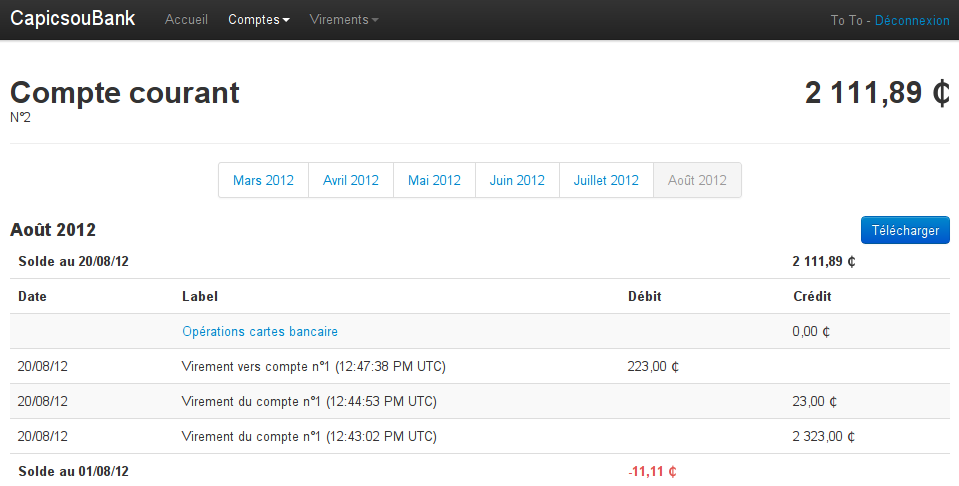
\includegraphics[width=\linewidth]{images/capicsoubank.pdf}
	\caption{Résumé du compte pour le mois d'août}
\end{figure}

L'application est disponible à l'adresse : \url{http://capicsoubank.j.layershift.co.uk}. Pour se connecter, on peut utiliser le compte avec le nom d'utilisateur \verb+toto+ et le mot de passe \verb+toto+.\\

Cette application nous aura permis de terminer notre formation, en nous faisant la main sur les technologies les plus utilisées dans le monde de l'entreprise. Cette application nous a aussi forcé à faire attention à la façon d'implémenter certains aspects d'une application web, notamment à faire attention aux nombres de requêtes par page.\\

Bien que nous n'avions aucun impératif de performance, nous nous sommes restreints au strict nécessaire en terme d'accès base de données pour garantir un bon fonctionnement, même avec une charge sur le serveur.\\

Enfin, l'utilisation des méthodes Agiles nous a permis de développer rapidement sans avoir le réflexe de tout prévoir avant de véritablement implémenter les fonctionnalités. Avec les méthodes Agiles et toutes les méthodes fonctionnant en itération, il ne faut pas développer plus que nécessaire pour la fonctionnalité en cours. L'avantage est de ne pas avoir de code qui sera peut être utilisé plus tard et qui, en réalité, deviendra très certainement du code mort.
